\section{Results: Survey}\label{section:Results_Survey}

\subsection{Population Selection}
We initially had two sources for our Experienced Drools users to send our survey to.
From LinkedIn we selected users who were at one degree of separation from us and listed Drools in their skills.
From StackOverflow we selected users who had asked or answered questions about Drools.

As in these two websites the users do not tend to list their contact details, some investigation was required.
From the initial selection, whose size we did not record we harvested email accounts, and failing that twitter accounts.

A few days into our survey we read a paper that described the use of academic papers as a population of expertise.
We used Google Scholar to look up Drools papers from the previous 2 years.
After skimming the papers to ensure that it was specifically about or using the Drools language we harvested emails

On the second and fourth day of the survey two subjects forwarded the weblink to the survey to mailing lists.
One, a developer from the core Drools team, sent it to a list of known Drools consultants.
The other sent it internally in his company.
both the subjects who sent the survey to their mailing list forwarded links to version C of the survey.

We had created 4 versions of the questionnaires to a combat single source bias.
We distributed the surveys to the subjects harvested from LinkedIn and StackOverflow evenly.
Because of the overrepresentation of Survey C, we distributed the subjects harvested from academic papers evenly over Surveys A, B and D.

The collection result can be seen in figure \ref{fig:Survey_participants}.
What we see here is that the method of collection did not have much of an impact on return rates.
whilst StackOverflow had a higher rate, the number of people contacted was so small that a small addition of respondents has an outsized effect on the proportion.

The first three pie charts represents the collection methods over which we had control.
These three represented 24 of our 30 completed questionnaires.
The last pie chart represents 6 completed and 4 partially completed questionnaires, that were returned from the surveys sent on by our initial participants.
We do not know the size of the starting population of these lists. 
Thus this pie chart only shows the ratio of partial to completed results.


In summary, a survey reached known 154 participants, of which 24 completed it, for a Response Rate of 15.5\%.
In addition, an unknown amount of participants were reached through mailing lists, returning a further 6 completed surveys.

\subsection{Participant demography}

Responses came from around the world.
Figure \ref{fig:Survey_locations} shows the location of the respondents were concentrated in Europe, the exceptions being the USA, Israel, and Singapore.
Italy and the Netherlands provided the largest number of responses, with 7 and 5 respectively.

\begin{figure}[H]
    \centering
    \fbox{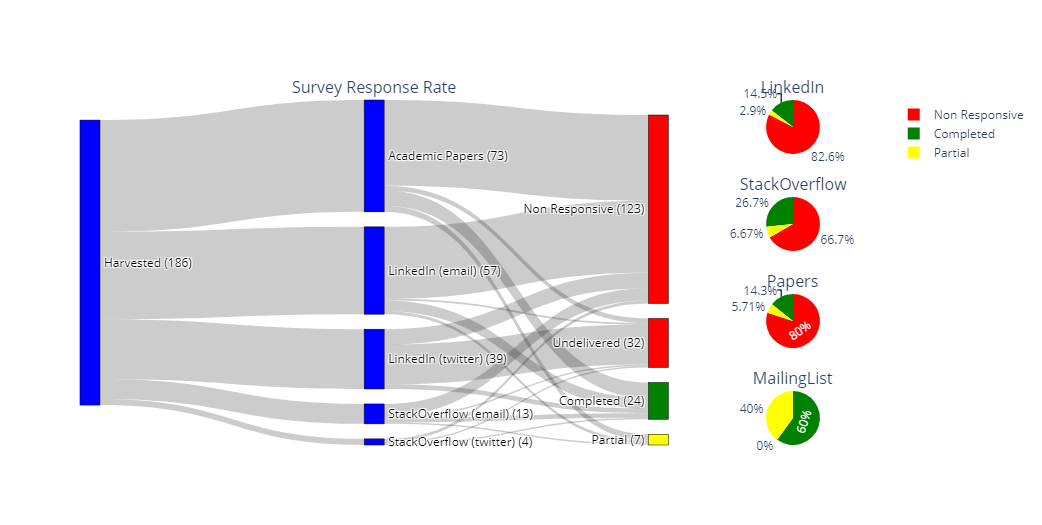
\includegraphics[width=0.95\textwidth]{Sections/images/survey_participants.png}}
    \caption{Survey Participants}
    \label{fig:Survey_participants}
\end{figure}

\begin{figure}[H]
    \centering
    \fbox{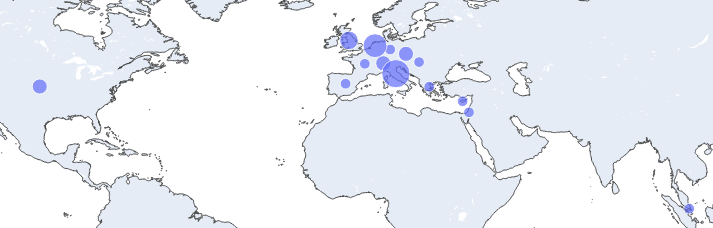
\includegraphics[width=0.95\textwidth]{Sections/images/survey_locations.png}}
    \caption{Survey Locations}
    \label{fig:Survey_locations}
\end{figure}

\begin{figure}[H]
    \begin{subfigure}{.33\textwidth}
      \centering
      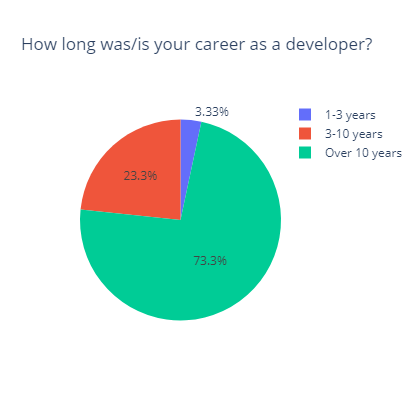
\includegraphics[width=.95\linewidth]{Sections/images/pie_experiencer.png}
      \caption{a}
      \label{fig:sfig1}
    \end{subfigure}%
    \begin{subfigure}{.33\textwidth}
      \centering
      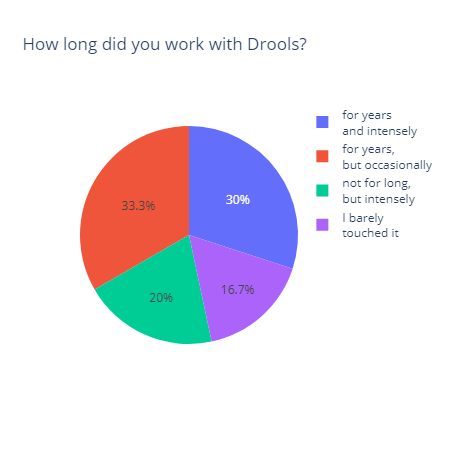
\includegraphics[width=.95\linewidth]{Sections/images/pie_droolsExperience.png}
      \caption{b}
      \label{fig:sfig2}
    \end{subfigure}
    \begin{subfigure}{.33\textwidth}
        \centering
        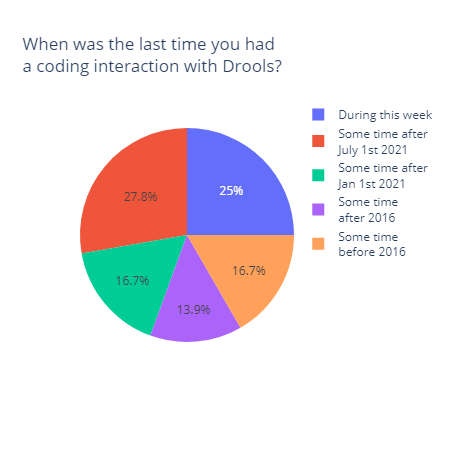
\includegraphics[width=.95\linewidth]{Sections/images/pie_recentusage.png}
        \caption{c}
        \label{fig:sfig3}
      \end{subfigure}
    \caption{Subject Experience}
    \label{fig:subject_experience}
\end{figure}

The experience of our subjects was quite high.
As can be seen in \ref{fig:subject_experience}, most of our subjects have over 10 years programming experience.
17\% of our recipients had a low experience of Drools, and 30\% were very experienced.
Over half of our recipients have used Drools in the previous 6 weeks with only 17\% not having used Drools for more than 5 years.

